\documentclass{ximera}

\title{What is a limit}

\newenvironment{objectives}{\begin{remark}\textbf{Objectives}}{\end{remark}}

\begin{document}
\begin{abstract}
\end{abstract}

\maketitle


\begin{objectives}


\begin{itemize}
   \item What is a limit
   \item What is a one-sided limit
    \item When does a limit not exist
    \item What does it mean for a function to be continuous
    \item If we know a function is continuous, how can this help us find a limit
\end{itemize}

Computational goals

\begin{itemize}
    \item Calculate limits from a graph (or state that the limit does not exist)
    \item Estimate limits using nearby values
    \item Find interval of continuity
    \item Use continuity to evaluate limits
\end{itemize}


\end{objectives}

\section{Finding Limits Graphically}
\subsection{Lesson What is a limit}

\begin{center}  
\youtube{U1PxqDjVfBQ}  
\end{center}

\subsection{Quiz}

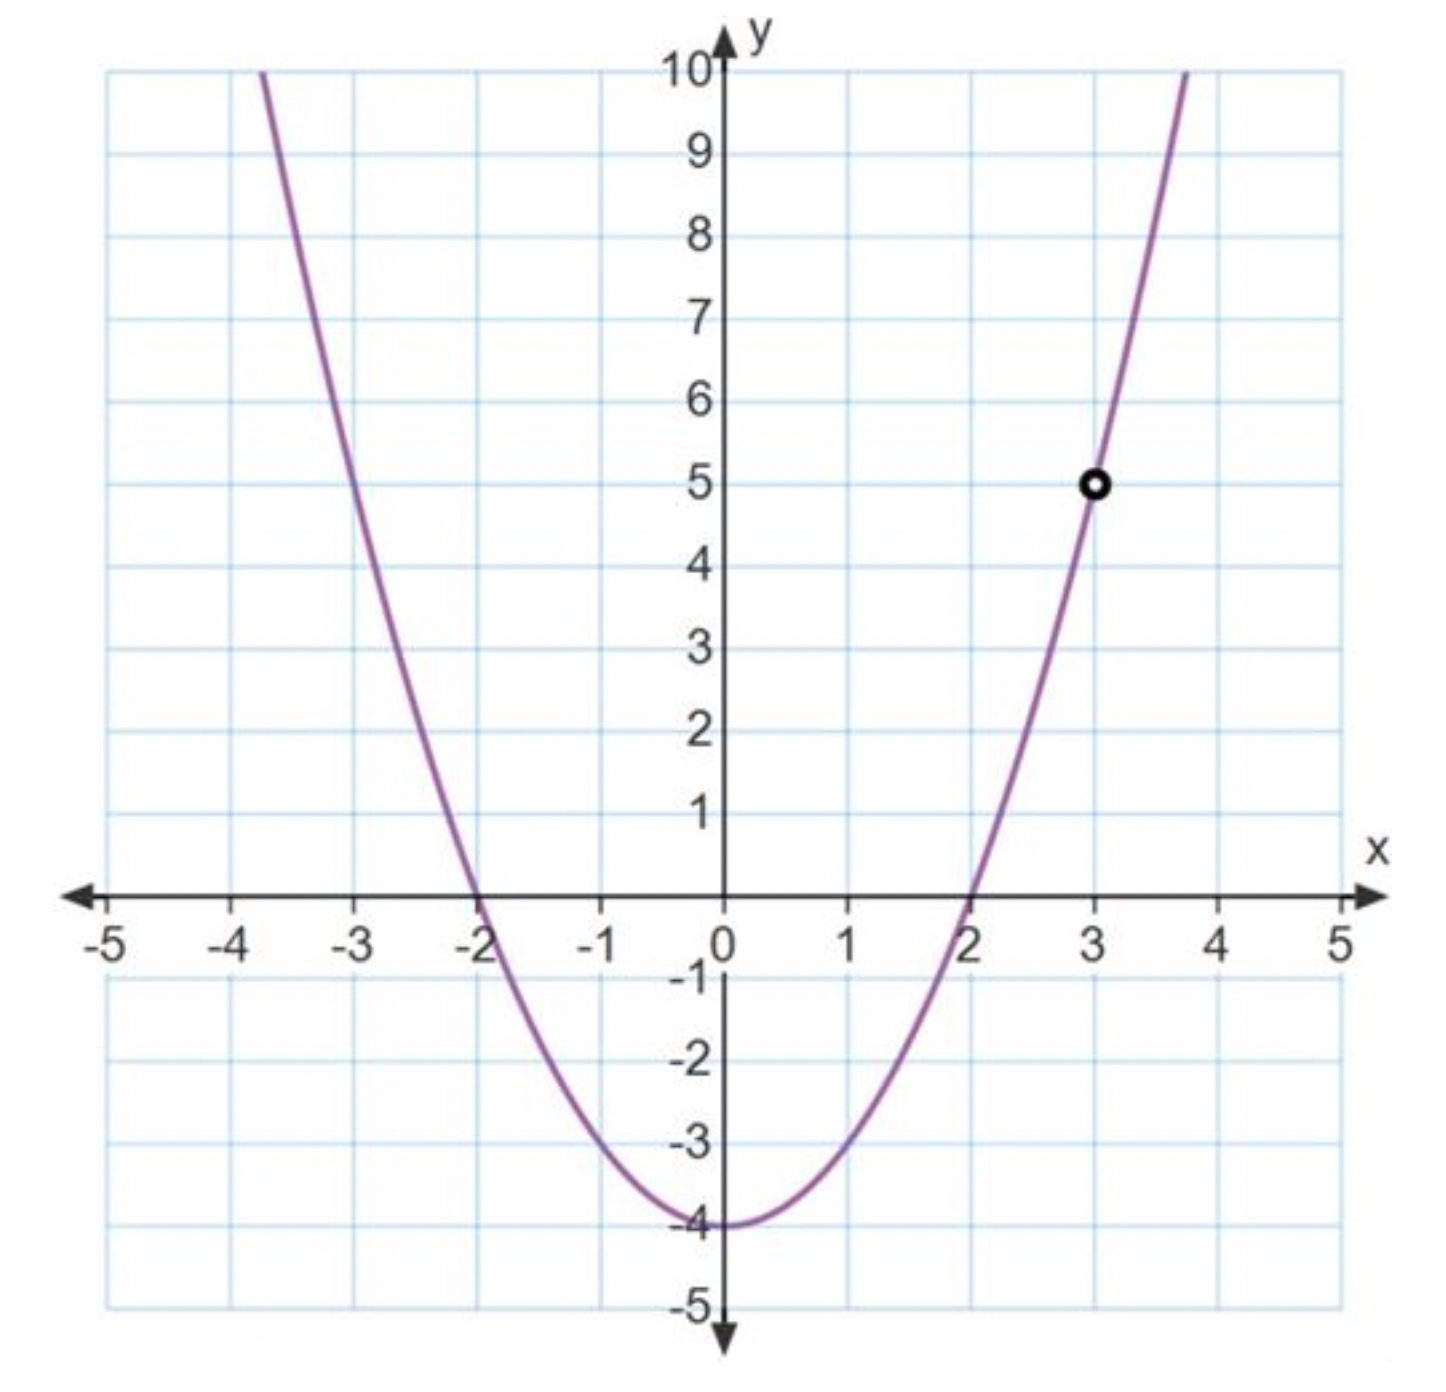
\includegraphics[width=0.5\textwidth]{graph1.png}
\begin{question}  
$\lim_{x to 3} f(x) = \answer{5}$  

% begin{exploration}
\begin{explanation}
    That's right! You selected the correct response. The limit as $x$ approached $3$ is $5$. This is the $y$-value the graph is getting close to when the $x$-value is near $3$.
% end{exploration}
\end{explanation}
\end{question}


\section{Finding Limits Numerically}
\subsection{Lesson Evaluating a rational function}
\begin{center}
\youtube{YTKoob7m3DM&t=36s}
\end{center}

The computation we just did plugged 3 into $f(x)$ and tells us $f(3)$. It does not necessarily tell us $lim_{x to 3} frac{x^2-1}{x-1}$.

Since the limit is supposed to be telling us what the $y$-value is near when $x$ is near $3$, we can estimate this by plugging in numbers near $3$, such as
\[
    2.9, 2.99, 2.999, \ldots, 3.001, 3.01, 3.1
\]

(eventually the following should link the correct subpages)
\begin{itemize}
    \item \link[I need a lot of help]{whatisalimit} Watch a video about estimating limits by checking nearby numbers.
    \item \link[I need a little help]{whatisalimit} Watch a shortened video.
    \item \link[I think I understand]{whatisalimit} Skip to the quiz.
\end{itemize}


\subsection{Estimating limits video}
\begin{center}
\youtube{sM4lzNqAdiA}
\end{center}

\subsection{Estimating limits video (short)}

\begin{center}
\youtube{sM4lzNqAdiA&t=185s}
\end{center}

\subsection{Quiz}

\begin{question}  
Which of the following statements is \underline{true} regarding the relationship between the limit as $x$ goes to $a$ of $f(x)$ and $f(a)$  That is, the relationship between the limit and the function value at the point $x=a$. (You should have 2 attempts; not sure if there's a way to do this in Ximera.)
\begin{multipleChoice}  
\choice{The limit of $f(x)$ as $x$ goes to $a$ and the function value $f(a)$ always give the same value because the function must be approaching its function value.}
\choice{The limit of $f(x)$ as $x$ goes to $a$ and the function value $f(a)$ always give different values since they are by definition different quantities.}
\choice[correct]{The limit of $f(x)$ as $x$ goes to $a$ and the function value $f(a)$ are by definition different quantities. They may or may not have the same numerical value, depending on the behavior of $f(x)$ near $x=a$.}  
\end{multipleChoice}  

% begin{exploration}
\begin{explanation}
    That's right! The limit of $f(x)$ as $x \to a$ and the function value $f(a)$ are by definition different quantities. They may or may not have the same numerical value, depending on the behavior of $f(x)$ near $x=a$.
% end{exploration}
\end{explanation}
\end{question}

\subsection{Lesson Estimating limits from nearby numbers}
\begin{center}
    \youtube{YTKoob7m3DM&t=150s}
\end{center}

What would you like to do next
(eventually the following should link the correct subpages; maybe put them in expandable environments)
\begin{itemize}
    \item \link[See how to find this limit graphically.]{whatisalimit} 
    \item \link[See another example of limits estimated with a table.]{whatisalimit}
    \item \link[Continue the lesson and learn about one-sided limits.]{whatisalimit}
\end{itemize}

\subsection{Example Finding a limit graphically}
\begin{center}
    \youtube{why41NH7U4k}
\end{center}

\subsection{Example Estimating a limit using nearby values}
\begin{center}
    \youtube{C-xihdPs9s}
\end{center}

\section{One-Sided Limits}

We can extend these same concepts and definitions to the idea of a one-sided limit...

$\lim_{x to a^+} f(x)$ means ``What value does $f(x)$ approach as $x$ approaches $a$ only from the right side''

$\lim_{x to a^-} f(x)$ means ``What value does $f(x)$ approach as $x$ approaches $a$ only from the left side''

\subsection{Lesson one-sided limits}

\begin{center}
    \youtube{KI5tjq2yrcI}
\end{center}

\subsection{Practice problem}

Take a few minutes to practice by evaluating the following (this is not graded; click to reveal answers)

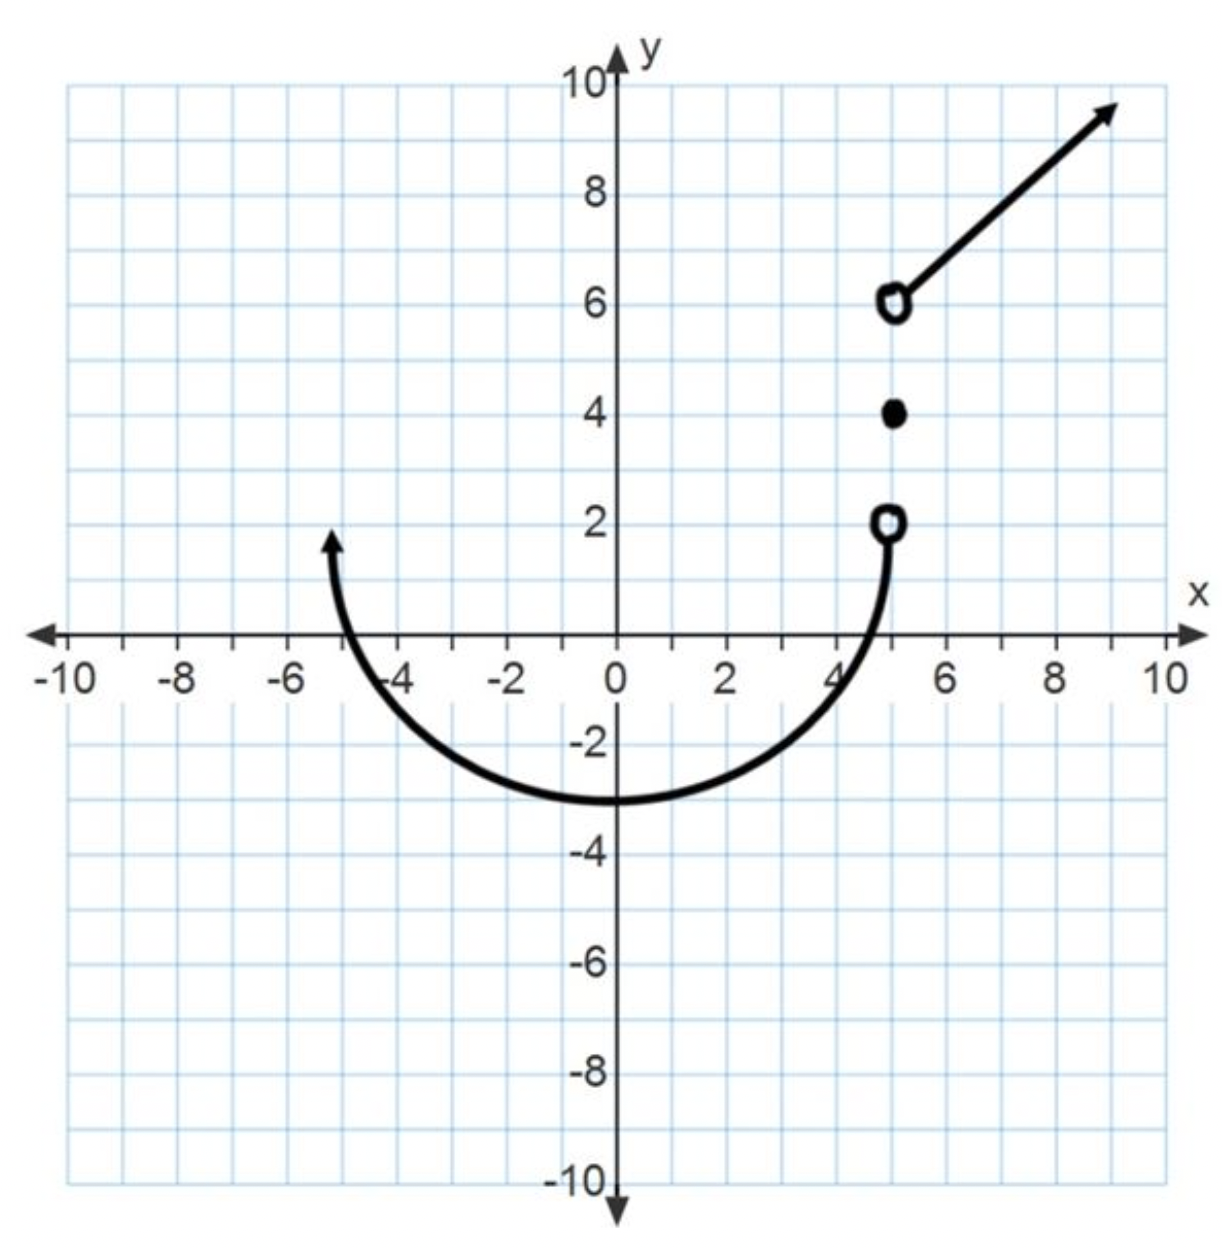
\includegraphics[width=0.5\textwidth]{graph2.png}

\begin{itemize}
    \item $f(5)$
    \begin{expandable}
        Value $4$
    \end{expandable}
    \item $\lim_{xto5^+} f(x)$
    \begin{foldable}
        Value $6$
    \end{foldable}
    \item $\lim_{xto5^-} f(x)$
    \begin{expandable}
        Value $2$
    \end{expandable}
\end{itemize}

\section{Limits which ``Do Not Exist''}

Sometimes, a limit may not exist.

\begin{explanation}
    A limit does not exist if $f(x)$ does not approach a single value as $x$ approaches $a$.
\end{explanation}

We use the notation DNE (which stands for ``Does Not Exist'') when a limit does not exist.

Use the links below to explore three scenarios in which the limit does not exist (all three should be required; not sure how to do this in Ximera). After you have explored all three, click to complete the assessment.

\subsection{Oscillations}
\begin{center}
    \youtube{EoT5FZdt6qs}
\end{center}
\subsection{One-sided limits do not match}
\begin{center}
    \youtube{KI5tjq2yrcI&t=131s}
\end{center}
\subsection{Infinite limits}
\begin{center}
    \youtube{gCuh1DmvvQE}
\end{center}
\subsection{Assessment}
\begin{question}
What is the limit of the pictured function as $x$ approaches $5$ (You have 2 attempts.)

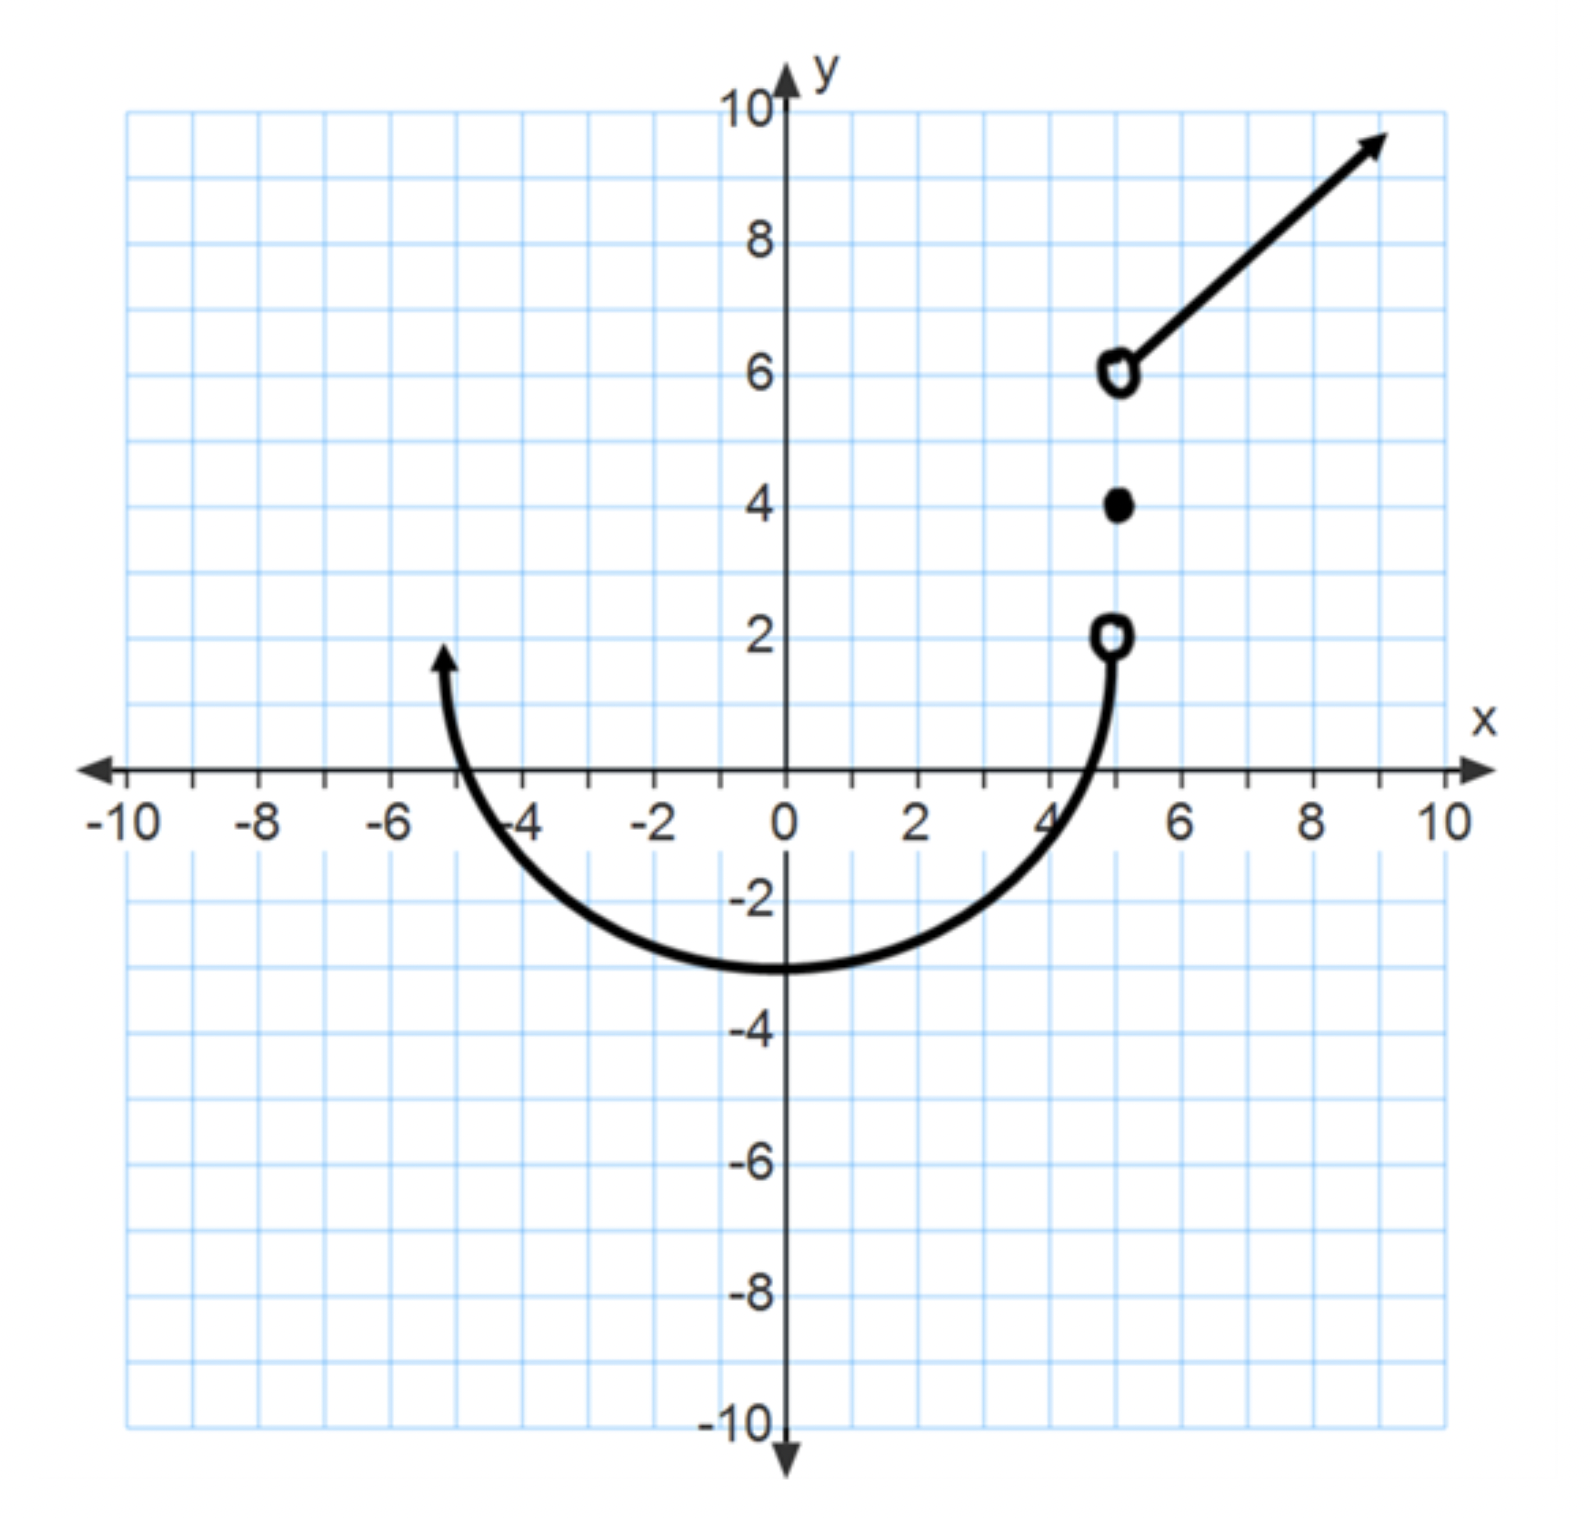
\includegraphics[width=0.5\textwidth]{graph3.png}
\begin{multipleChoice}  
\choice{4}
\choice{DNE}
\choice[correct]{2}  
\choice{6}
\end{multipleChoice}  

\begin{explanation}
    That's right! The correct response is DNE. While the one-sided limits do exist, the limit as $x \to 5$ of this function does not exist because the one-sided limits are not equal.
\end{explanation}
\end{question}

\section{Continuity}

\subsection{Lesson Continuity at a point}

\begin{center}
    \youtube{ReDZpc5jhCw}
\end{center}

\subsection{Requirements for continuity}

In order for the function $f(x)$ to be continuous at a point $x=a$, the following conditions must be met
\begin{enumerate}
    \item $f(a)$ is defined
    \item $\lim_{x to a} f(x)$ exists
    \item $\lim_{x to a} f(x) = f(a)$ (the function value and limit are equal at $a$).
\end{enumerate}

\begin{explanation}
    \begin{foldable}
        \textbf{Intuitive vs. Formal Definitions.} Intuitively, the graph of $f$ is continuous at the point $a$ if the graph near $a$ can be traced ``without lifting your pencil''. While this way of thinking about continuity can be helpful to us in understanding the concept, it is not the mathematical definition. If you are asked to show a function is continuous at a point, you must use the mathematical definition given above!
    \end{foldable}
\end{explanation}

\subsection{Quiz criteria for continuity}

\begin{question}
Which of the following is NOT a criteria for continuity at $x=a$ (You have one attempt.)
\begin{multipleChoice}  
\choice{The function is defined at the point $x=a$}
\choice{The limit as $x$ approaches $a$ exists}
\choice{The limit as $x$ approaches $a$ is equal to the function value at $a$}
\choice{The function has no sharp turns or oscillations near $x=a$.}
\end{multipleChoice} 

\begin{explanation}
     That's right! The function has no sharp turns or oscillations near $x=a$ is not required for continuity.
 \end{explanation} 
\end{question}

\section{Continuity on an Interval}

Now that we've studied continuity at a point, let's expand our knowledge and learn what it means for a function to be continuous on an interval $[a,b]$

\subsection{Lesson}
\begin{center}
    \youtube{ReDZpc5jhCw&t=213s}
\end{center}

To summarize...

\begin{explanation}
    \begin{foldable}
        \begin{itemize}
            \item The function $f(x)$ is continuous from the left at point $a$ if $\lim_{x to a^-} f(x) = f(a)$
            \item The function $f(x)$ is continuous from the right at point $a$ if $\lim_{x to a^+} f(x) = f(a)$
        \end{itemize}
        \begin{center}            
        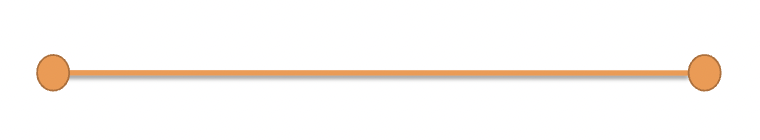
\includegraphics[width=0.5\textwidth]{graph4.png}
        \end{center}
    \end{foldable}

    \begin{foldable}
        The function $f(x)$ is continuous on the open interval $(a,b)$ if it is continuous at all points of the interval
    \end{foldable}

    \begin{foldable}
        The function $f(x)$ is continuous on the closed interval $[a,b]$ if it is continuous on the open interval $(a,b)$ and if $lim_{x to a^+} f(x) = f(a)$ and $lim_{x to b^-} f(x) = f(b)$.
        In other words, $f(x)$ is continuous on the closed interval $[a,b]$ if it is continuous at all points of the interior $(a,b)$, left continuous at $x=b$, and right continuous at $x=a$.
    \end{foldable}{}
\end{explanation}

\subsection{Examples}

Pictured are the graphs of two functions which are continuous for all real numbers. The first is a polynomial and the second is the cosine function.

\begin{center}
    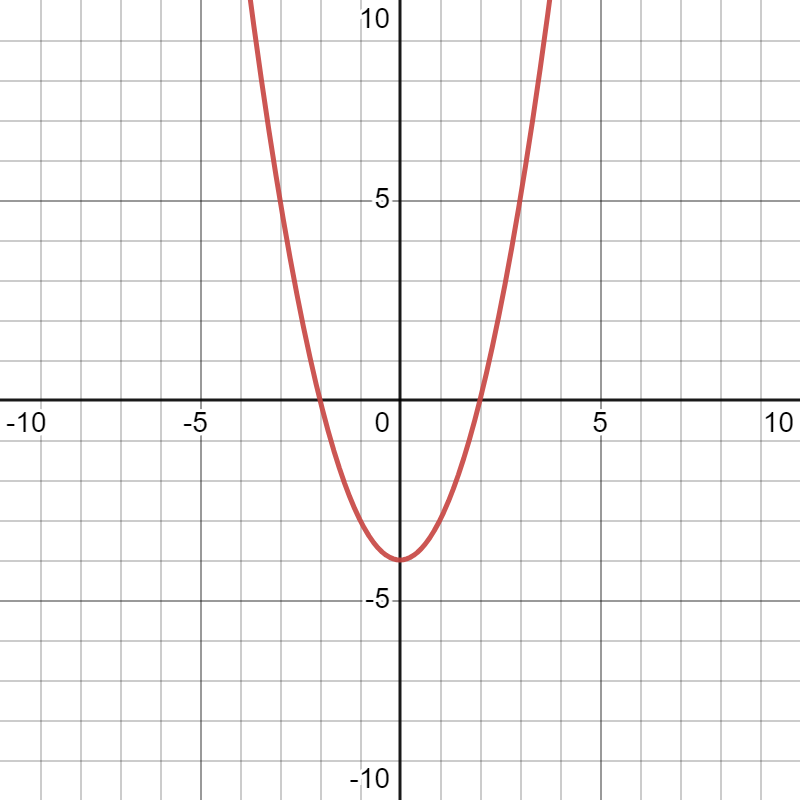
\includegraphics[width=0.75\textwidth]{graph5.png}
\end{center}

Below is an example of a discontinuous graph.

\begin{center}
    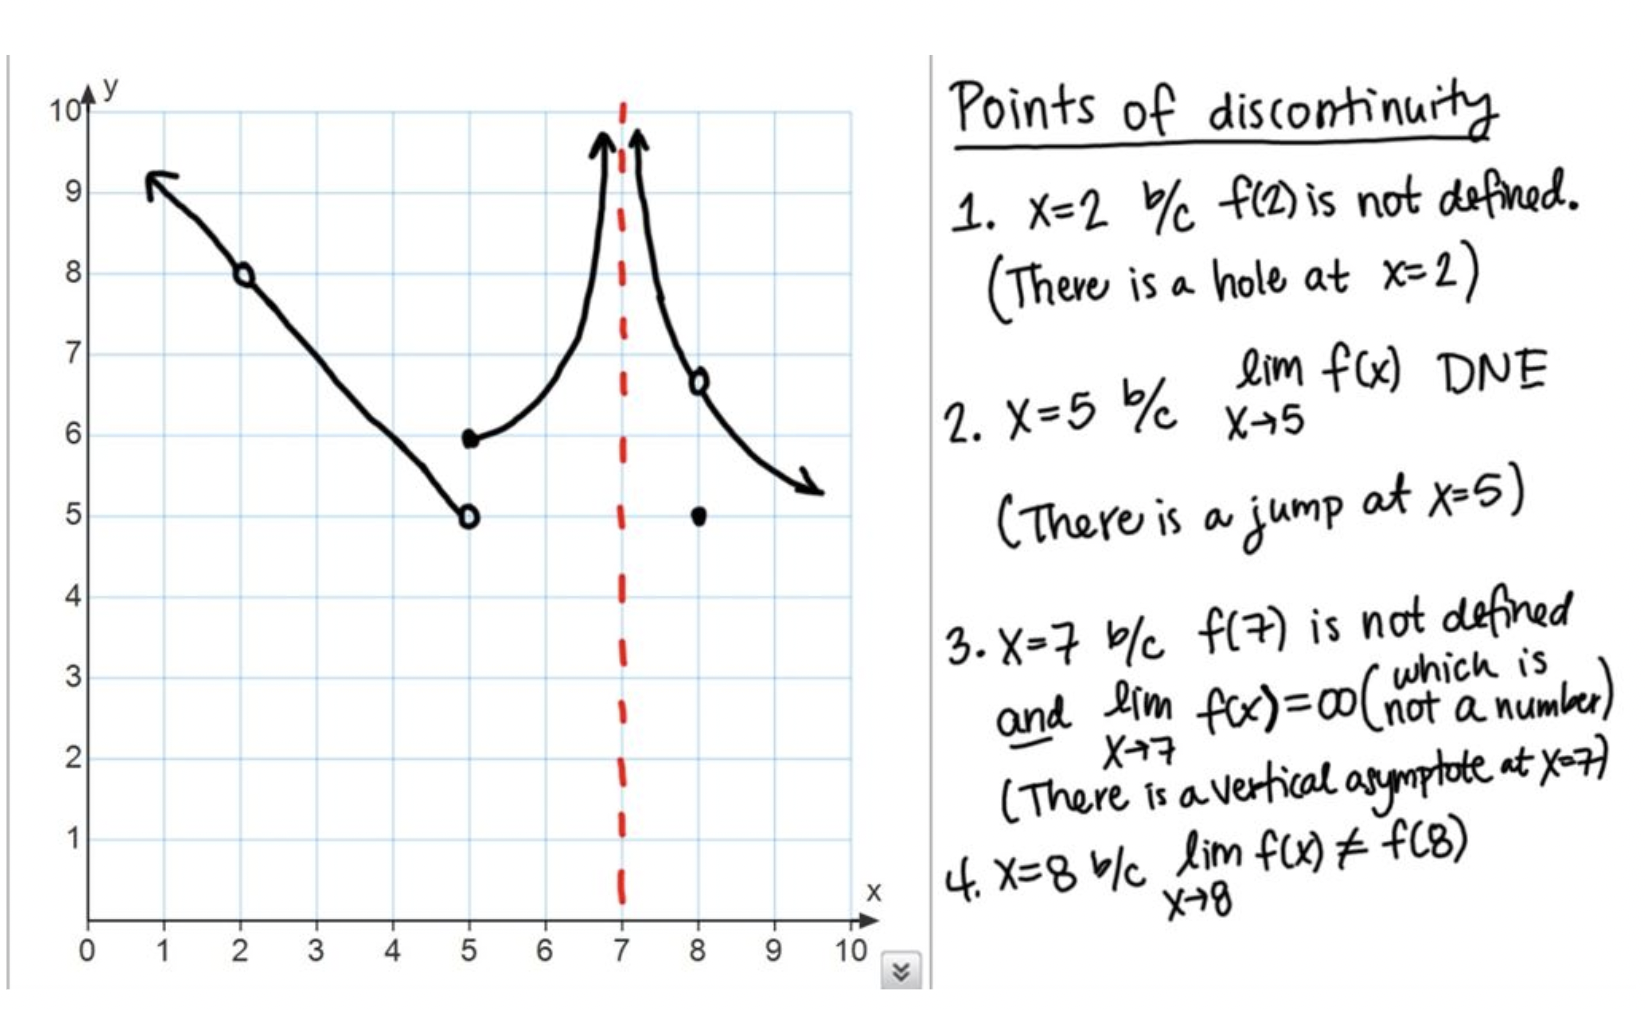
\includegraphics[width=\textwidth]{graph6.png}
\end{center}

\subsection{Famous functions}

\begin{theorem}
    The following functions are continuous on their natural domains, for $k$ a real number and $b$ a positive real number.
    \begin{itemize}
        \item Constant function \[f(x)=k\]
        \item Identity function \[f(x)=x\]
        \item Power function \[f(x)=x^b\]
        \item Exponential function \[f(x)=b^x\]
        \item Logarithmic function \[f(x)=log_b(x)\]
        \item Sine and cosine \[f(x)=sin(x), \qquad f(x) = cos(x)\]
    \end{itemize}
\end{theorem}

We can now take limits of these functions without having to guess by evaluating them at nearby numbers. We know that for all values of $a$ in the domain of these functions, we can find the limit as $x$ approaches $a$ just by plugging $a$ into the function!
\[
    \lim_{x to a} f(x) = f(a)
\]

\subsection{Quiz}

\begin{question}
Use continuity to find this limit \[ \lim_{x \to \pi} sin(x) \]
\begin{multipleChoice}  
\choice[correct]{0, because $sin(\pi) = 0$.}
\choice{0 because if we plug numbers near $pi$ like $3.1$, $3.14$, and $3.15$ into $sin(x)$, we get out very small values.}
\choice{We don't know how to find the exact value of this limit yet.}  
\end{multipleChoice}  

\begin{explanation}
    That's right! Since we know that $sin(x)$ is continuous at $x = \pi$, we know that the limit as $x \to \pi$ is equal to what we get when we plug $\pi$ into $sin(x)$.
\end{explanation}
\end{question}

\end{document}